
\section{Expedition Findings}

Our major cave finds this year can be considered in three separate
developments within \passage{Vrtnarija}:


\subsection{\texorpdfstring{The \passage{Serpentine} \& \passage{Let na Drugi
Svet}}{The Serpentine \& Let na Drugi Svet}}

An active streamway, named the \passage{Serpentine}, led off from a large
chamber (the \passage{Albert Hall}) discovered along \passage{Prince Consort
Road}. During 2010, this was pushed to -621 m (\passage{It Will Rain for a
Million Years}). Exploration in 2011 continued along this active
meander.

The initial exploration (\passage{Round Pond}) descended a 2 m climb down leading
to an oxbow and 4 m pitch. The following trip traversed out along a
crack in the ceiling to avoid falling water down a 10 m pitch
(\passage{Longwater}) which entered a chamber (also \passage{Longwater}) with
significant iron deposits (in the form of heavy $\approx$ 4 cm
thick plates of dark mineral in a vein within the limestone), and a
considerable number of orange-stained straws and stalactites.

\begin{marginfigure}
\checkoddpage \ifoddpage \forcerectofloat \else \forceversofloat \fi
\centering
 \frame{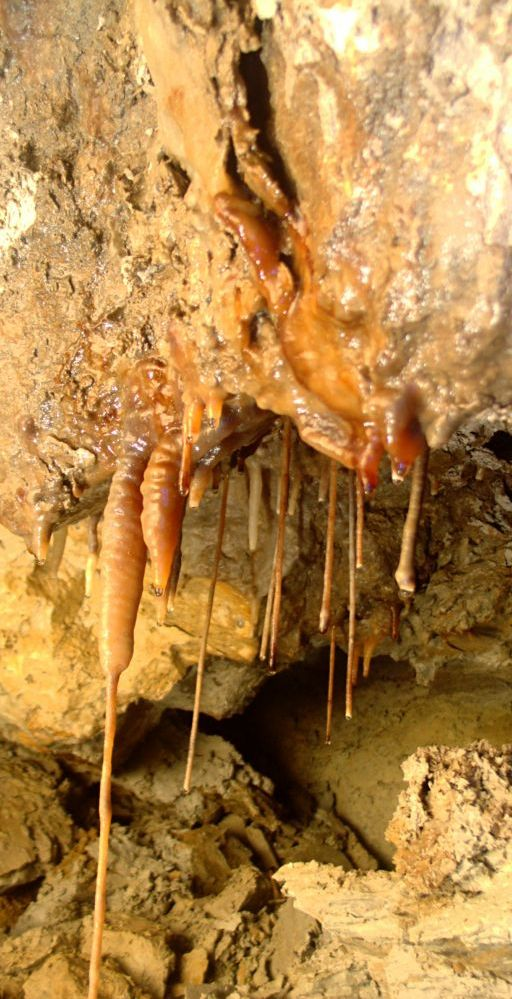
\includegraphics[width=\linewidth]{2011/discoveries/2011-08-06-04.57.28-Jarvist Frost-CanonG5-CRW_0154 - formations in the Long Water--orig.jpg}} 
 \caption{Formations in \protect\passage{Longwater}. \pic{Jarvist Frost}}  \label{longwater formations}
\end{marginfigure}

The boulder collapse in this chamber was bypassed by a squeeze between
boulders on the right which entered a crawl-way which soon refound the
water flowing from beneath the boulders. A 4 m pitch was reached where
the bedding plane appeared to intersect a joint. A 3 m diameter
apparently rather deep pool is present below this pitch. Passage
continues in vadose development with the water, which entered a small
chamber with a set of cascades (cascade chamber). There is also an
apparently phreatic connection between high up in the roof of this
cascade chamber and part way up the 4 m pitch.

The cascade chamber is rather complex in structure, the cascades falling
into a large \& deep 4x2 m pool. This water flows down a short rift and
immediately tumbles down a $\approx$ 8 m pitch (\passage{Duffers Drop})
which leads via two freeclimbable cascades (requiring very careful
maneuvering near to the water) to reach a wet inlet on a large pitch
(\passage{Drink Your Own}).

Behind the large pool in cascade chamber there is a dried pool with
haematite deposits and the start of a phreatic crawlway (\passage{Rotten
Row}), which is hidden from view unless you're crouching next to the
dried pool. This crawlway leads to a short pitch into the dry end of the
rift-developed \passage{Drink Your Own} pitch.

The cascade chamber also contains a rock bridge which can be used to traverse over the chamber into a dry scalloped shape alcove and so avoid climbing the direct 2 m cascade to the pool.

The maximum depth reached was -688 m. Our surveys indicate that the
current termination, at a large wet pitch with two accessible pitch
heads (via \passage{Duffers Drop}, or \passage{Rotten Row}), is very close to
the \passage{Republika} chamber at -723 m, where two streams enter from the
ceiling and split. Exploration was halted by the wetness of the pitch,
which will require a considerable effort in bolting to rig safely.
\passage{Drink Your Own} is a pitch which has developed in a perfectly
straight rift (probably fault controlled), with two streams entering the
rift from opposing perpendicular directions (i.e. perpendicular to the
rift direction of the pitch), one of which is the \passage{Duffers Drop} water
which we have been following continuously from the start of the
\passage{Serpentine} in the \passage{Albert Hall}.

The \passage{Serpentine} rope was derigged back to camp to avoid water
damage during winter.

The \passage{Serpentine} water flows continuously from the \passage{Albert
Hall} chamber to enter \passage{Drink Your Own} via \passage{Duffers Drop}.
The water entering on the opposite side of this large rift pitch is
considerably greater in volume and the source is unknown.

Below the first pitch in the \passage{Serpentine}, a climb was made to
access \passage{Let na Drugi Svet} (Fly to Another World), which via a
series of digs and a 21 m pitch led to a large active meander \passage{Krt
Kova Dobra Dela}\sidenote{\textbf{Little Mole Done Good}}, which is has been
pushed both upstream (to +19 m) and downstream (to -23 m) and is
ongoing. It is possible that this water forms the larger of the streams
that enters \passage{Drink Your Own}.

212 m of passage was found below \passage{It Will Rain}, and 252 m in
\passage{Let na Drugi Svet}.

\begin{marginfigure}
\checkoddpage \ifoddpage \forcerectofloat \else \forceversofloat \fi
\centering
 \frame{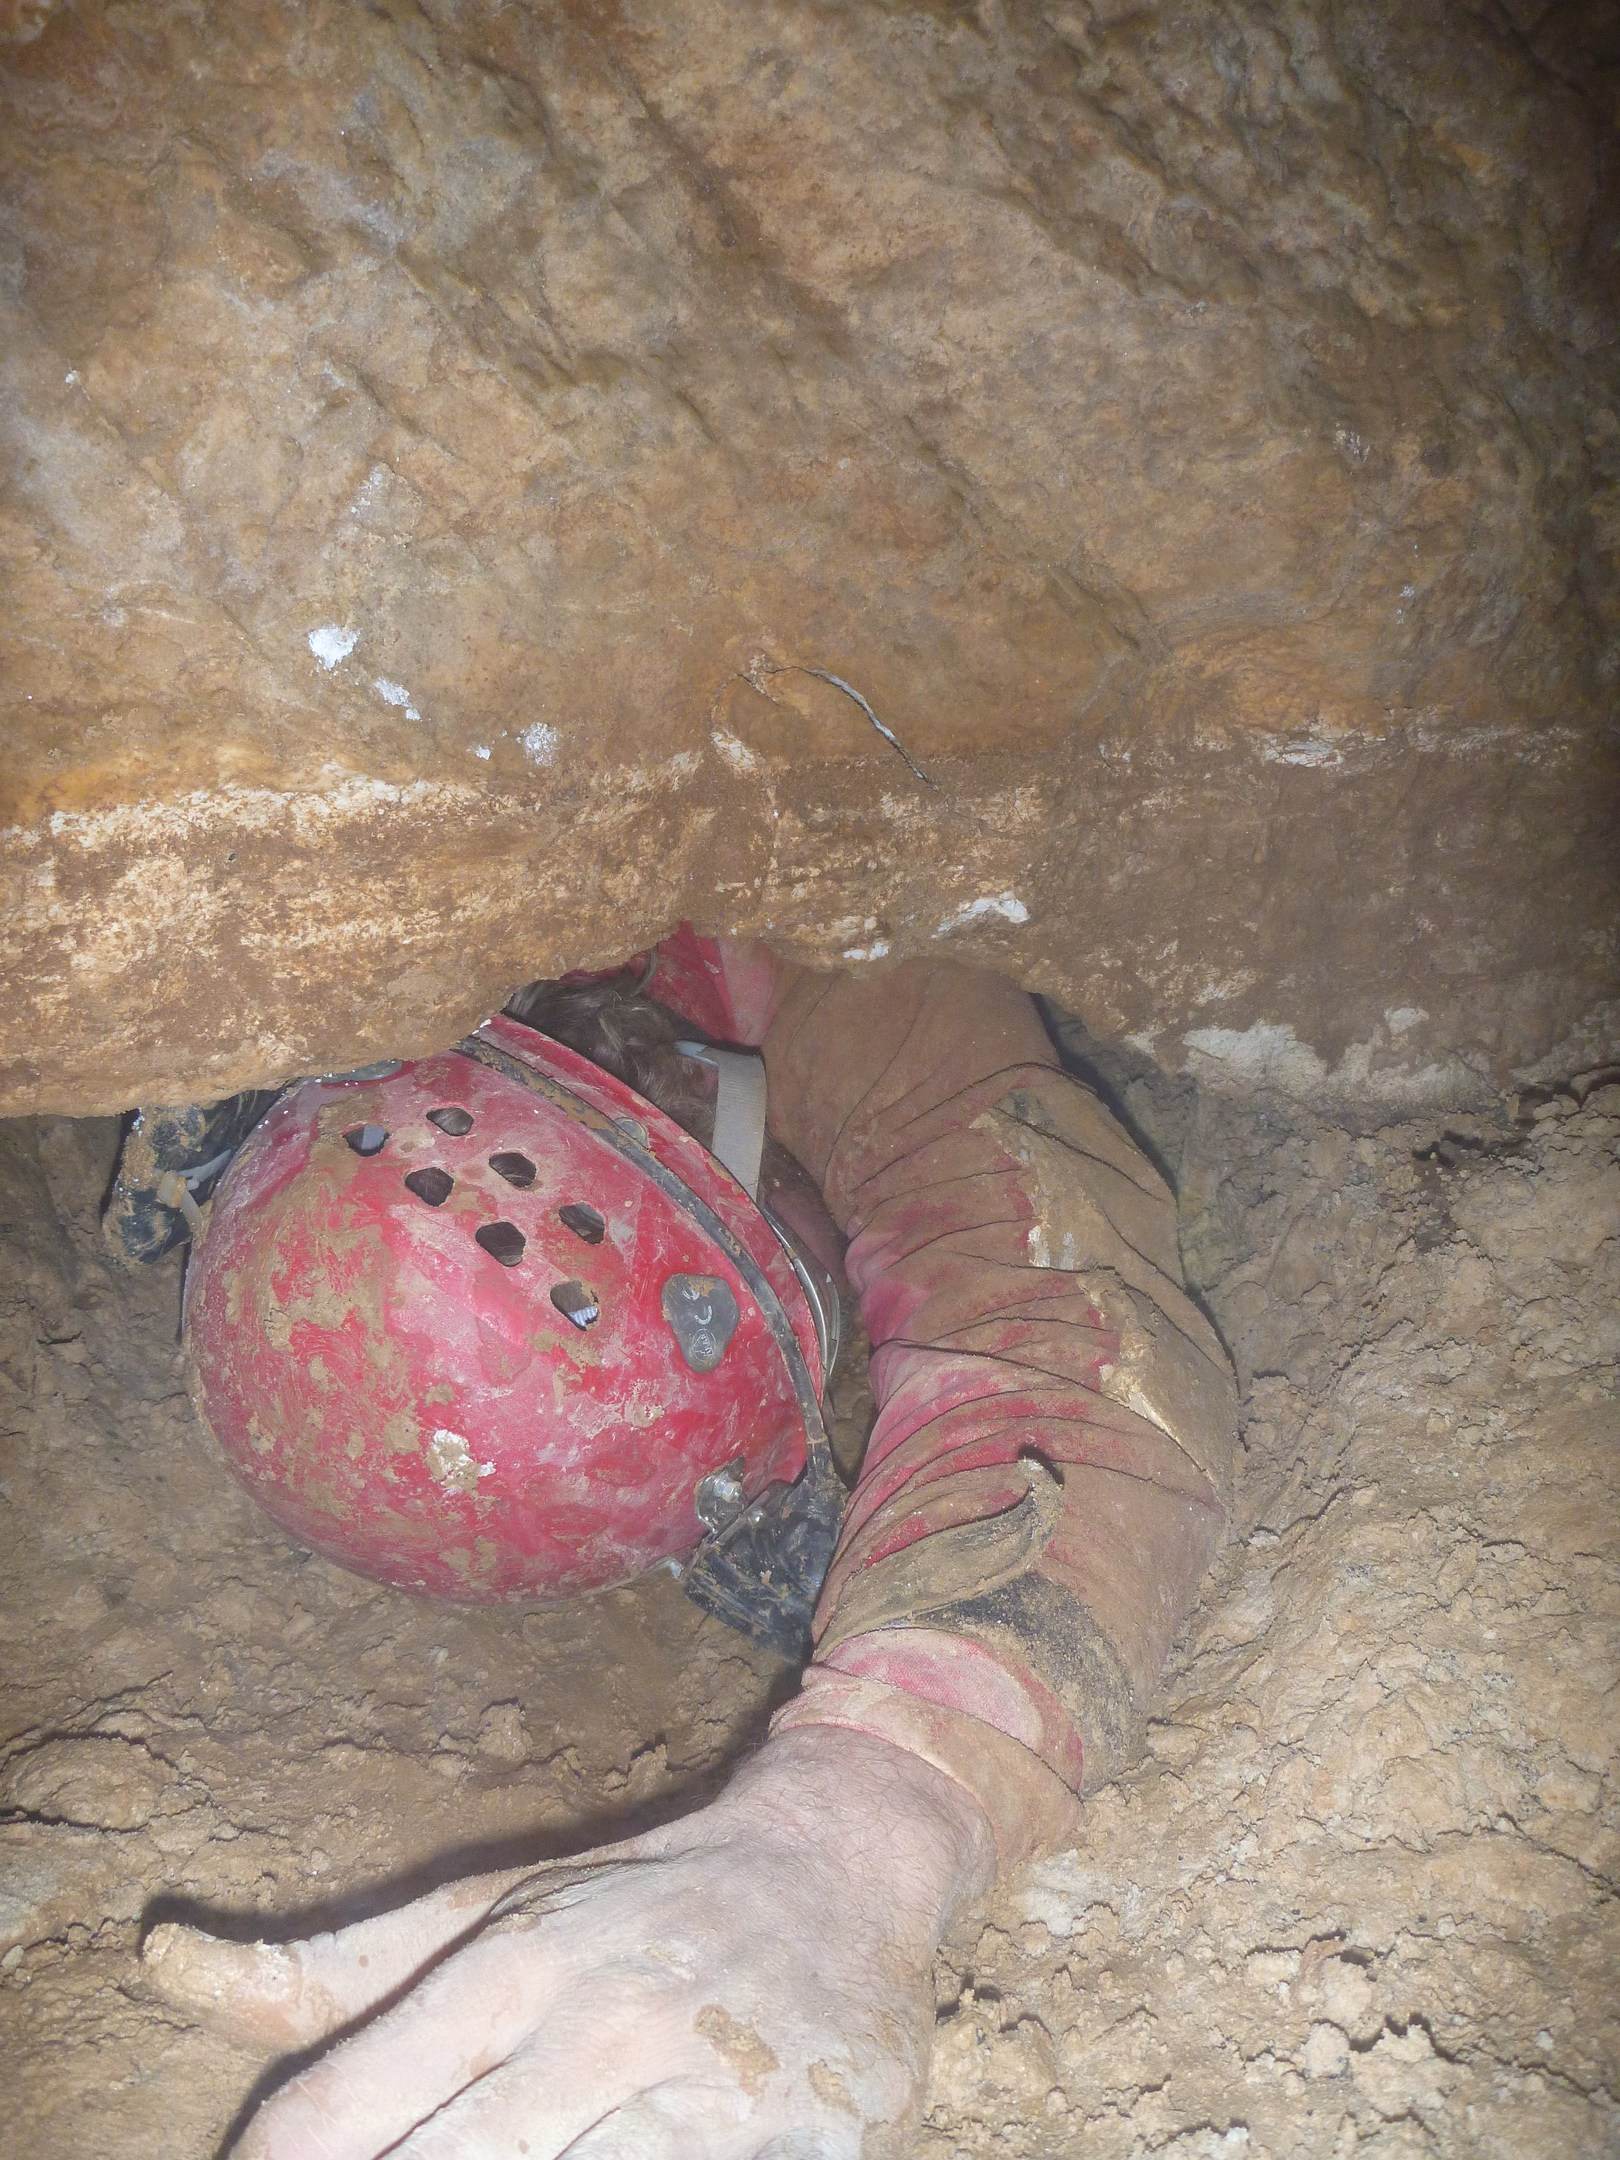
\includegraphics[width=\linewidth]{2011/discoveries/2011-08-01-19.11.24-Grega-Panasonc DMC-FT2-099-Let Na Drugi Svet--orig.jpg}} 
 \caption{Grega Maffi progressing through digs in \protect\passage{Let na Drugi Svet}. \pic{Tjaša Rutar}}
 \label{let na drugi svet dig 1}
\end{marginfigure}


\subsection{Insomnia}

\passage{Insomnia} is the continued exploration of a descending streamway
in the `deep' level of \passage{Vrtnarija} off Red Cow Roundabout, which
started with \passage{Republika} in 2009 and was left with an active
streamway at -802 m (\passage{Insomnia}, 2010). Two pushing trips
(\passage{Daydreamers}) followed this stream down a series of small (5-15
m) pitches. The last trip saw this stream disappear into a narrow,
too-tight, rift. A bypass was sought via an abandoned bedding plane
level (\passage{Penguin's Egg}), which gained the head of a chamber in which the
noise of falling water could be heard.

The descent and exploration of this chamber (\passage{Winter Journey}), found that
the loud stream noise could be heard through a too-tight rift formed in
a bedding plane with the characteristic -70 degree dip of the passages
near the sumps in \passage{SysMig}. This rift was also issuing a draught, which
was followed along the inclined bedding plane (heading North) through a
series of muddy squeezes to where it disappeared into an immature rift
in the roof. It is hypothesised that this could be the water-driven
draught return from a sumped section. The chamber had considerable thick
grey silt deposits, with unusual silt stalagmites on the boulders, which
may be evidence of a sump backing up.

The bedding plane was pushed in a northerly direction for circa. 20 m.
This is in the direction of the hypothesised dip of the mountain's water
table, and so it is possible that continued pushing or digging of this
bedding plane may lead to a sump bypass.

Exploration was carried out by trips that started on the surface
(confirming good weather for the day), went to the bottom, explored and
then returned to underground camp. This was due to us being extremely
concerned about the flood response of this new part of the cave. The
pitches are active, and due to a combination of the unavoidable cave
nature, and `exploration' rigging, they are wet even in moderate
conditions.

The 2011 exploration of \passage{Insomnia} found 294 m of passage and took
the cave to a new maximum depth of -888 m. The pitches were left fully
rigged as the intended last pushing trips did not occur due to a
multi-day rain storm near the end of expedition.


\begin{figure*}[t!]
\checkoddpage \ifoddpage \forcerectofloat \else \forceversofloat \fi
\frame{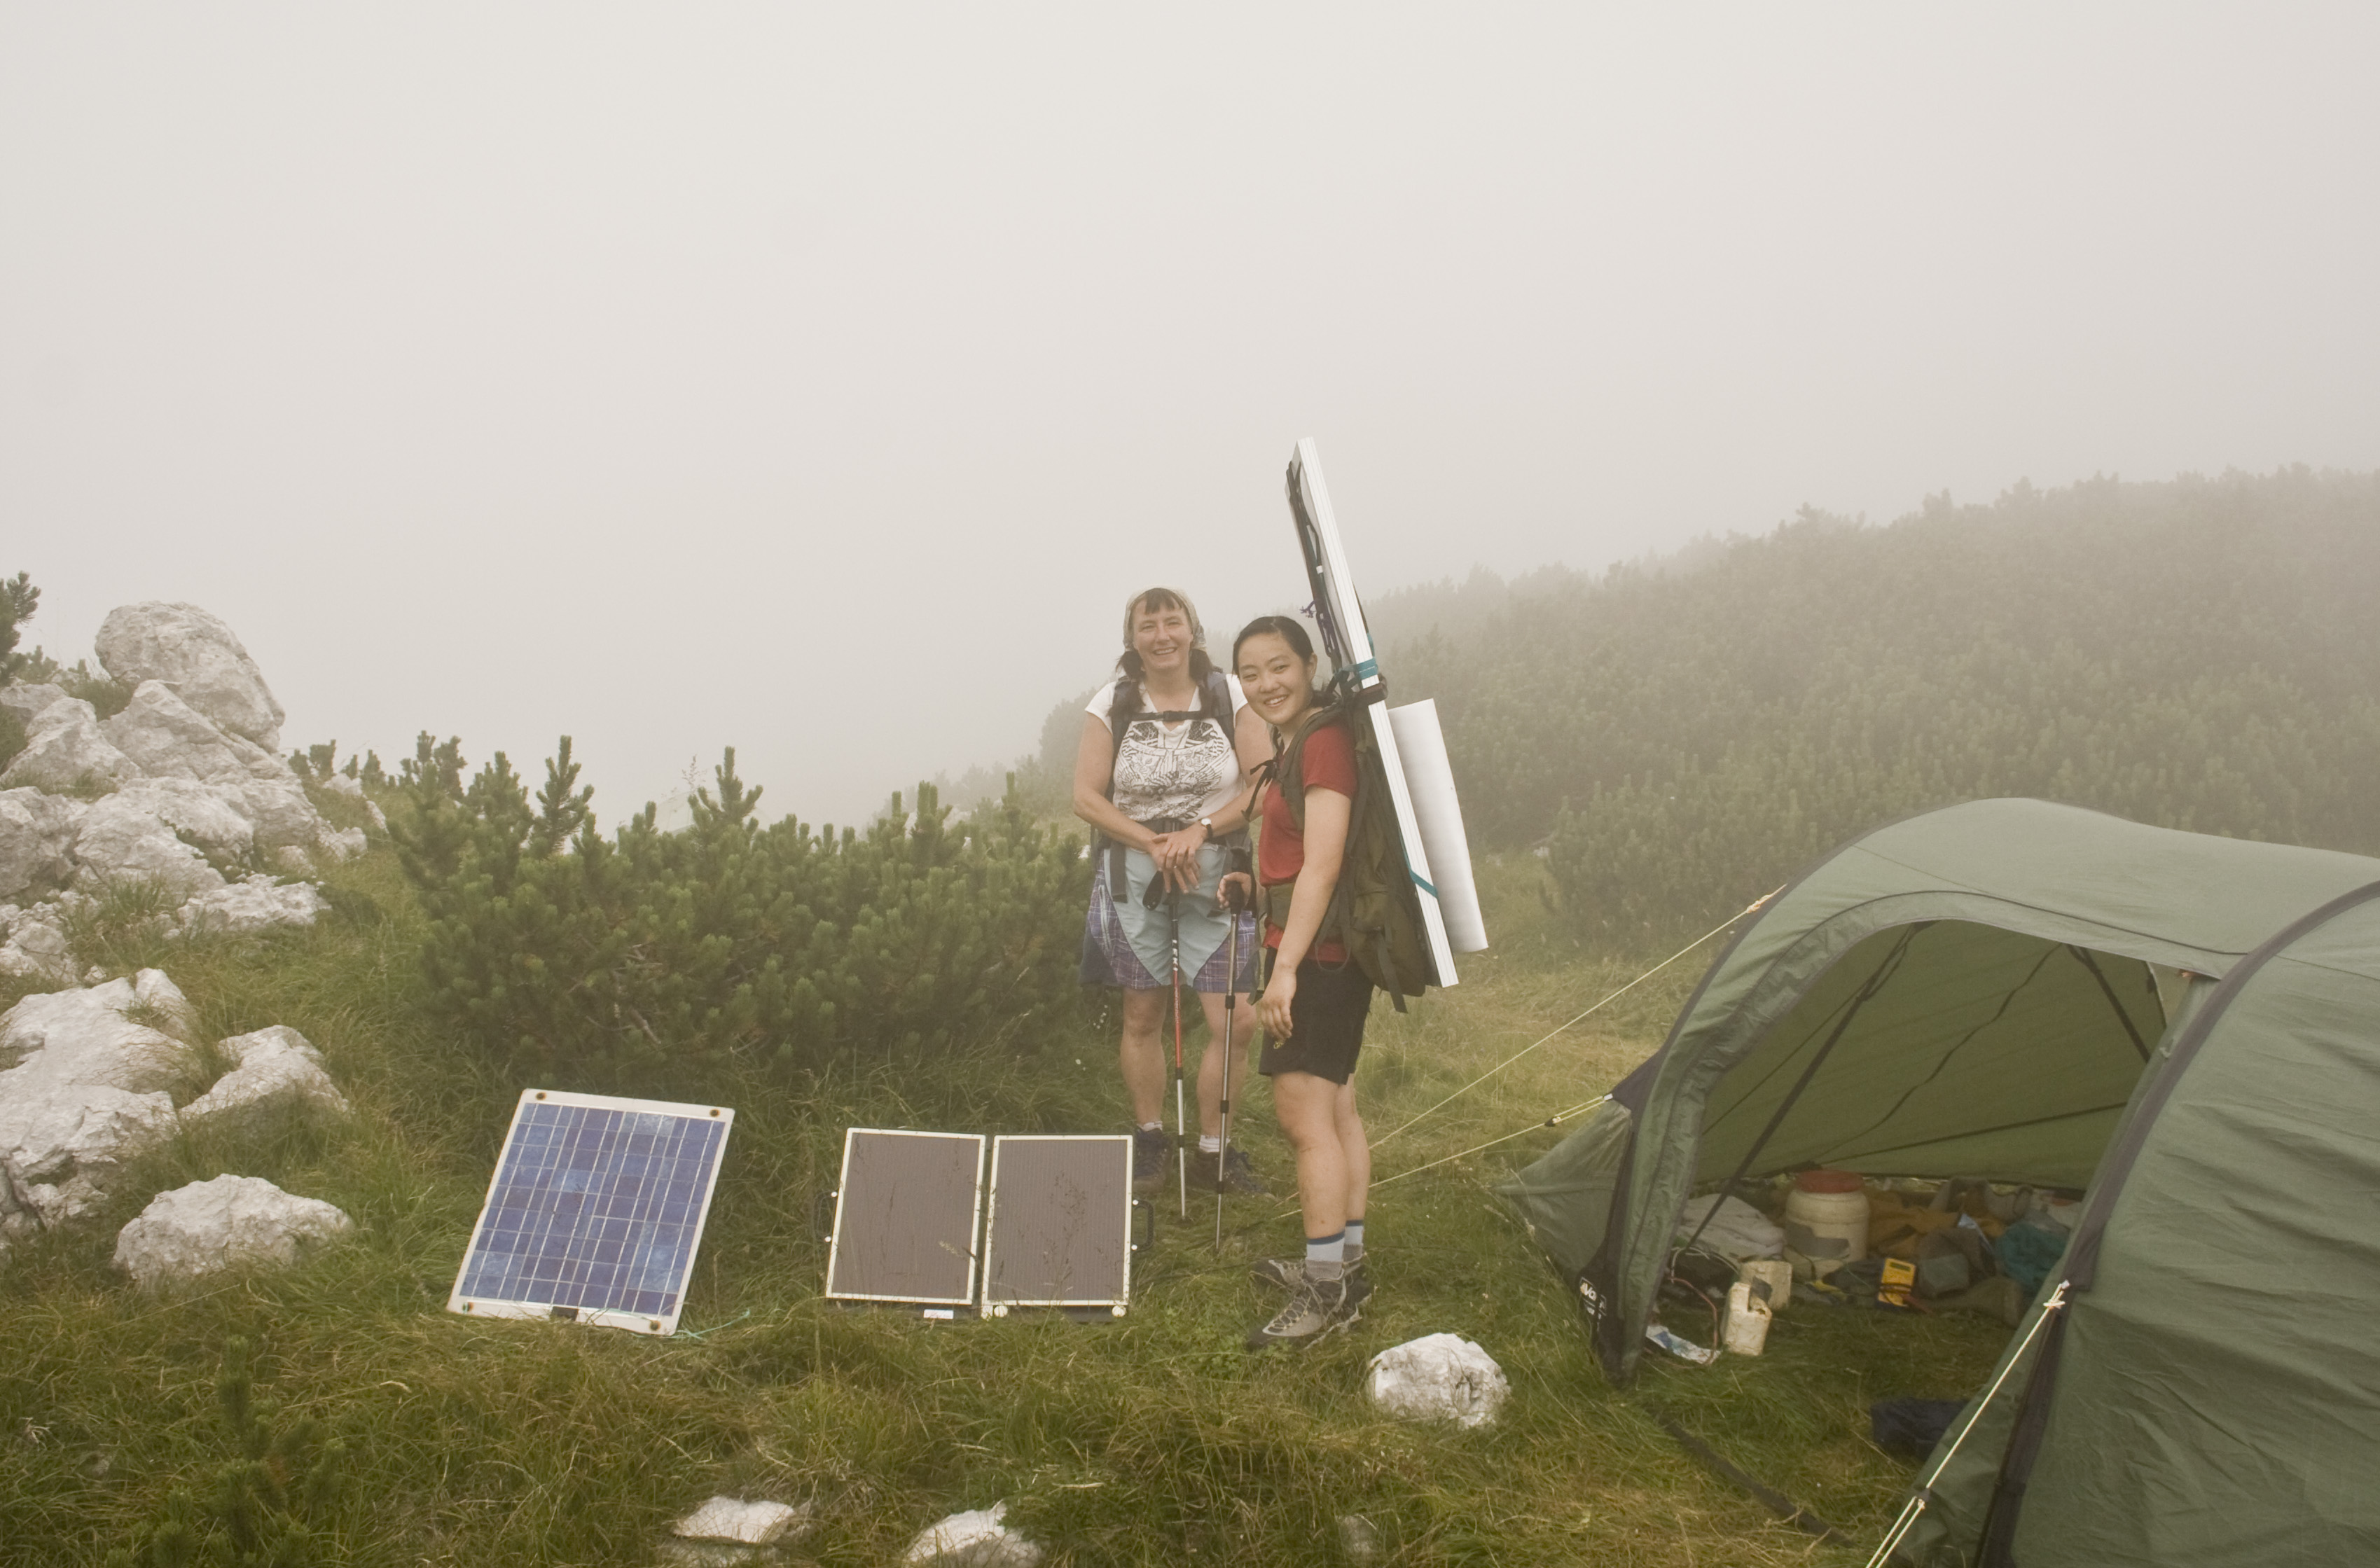
\includegraphics[width=\linewidth]{2011/discoveries/2011-08-04-12.28.43-Jana Carga-Canon 350D--orig.jpg}}
\caption{Janet Cotter and Clare Tan surrounded by the weather typical of \protect\passage[mountain]{Migovec} during the 2011 expo. Clare is carrying the new solar panel purchased using funds from the Wilhelm Putick Prize award. \pic{Jana Čarga}} \label{janet clare clag}
\end{figure*}





\subsection{Kamikaze}

\passage{Kamikaze} is a subtle route through the boulders on a ledge part
way down the pitch to \passage{Lost Hopes} in \passage{Wonderland} (the name given to
the chambers developing South / South East from \passage{Cheetah}). The
original explorer (DW) was making good use of his time while hand
bolting down the pitch continued, and the key squeeze through the
boulders was only found when \bignote{the condensation from an exasperated sigh
was noticed to disappear sideways!}

The sandy crawling passage was originally pushed upwind, to eventually
reach a boulder blockage in a spacious bedding plane beyond which a
large sound of water can be heard (\passage{Kamikaze}). There is enough
space in the bedding plane to dispose of boulder fragments, if it can be
reduced in size, and is an obvious future dig target.

This year we pushed downwind, almost instantly discovering a large
chamber (\passage{Red Baron}) and a bolt traverse over a pit to reach a
large ($\approx$ 6 m diameter) ascending (at almost exactly 30
degrees, in a straight line for 140 m) phreatic level (\passage{The Throne
Room}). This terminates in what appears to be a cross rift intersecting
it, making it a hammer head shape in plan. There is a 6 m undescended
pitch at the end, and the possibility of a traverse across this pitch
and a continuing crawl way.

\begin{marginfigure}
\checkoddpage \ifoddpage \forcerectofloat \else \forceversofloat \fi
\centering
 \frame{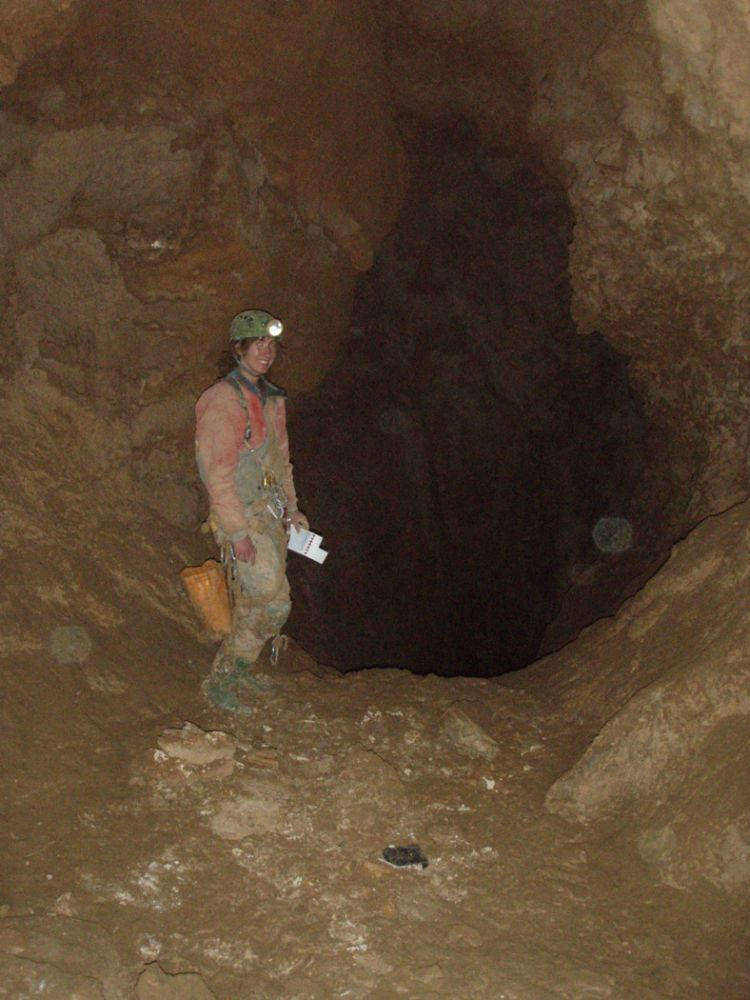
\includegraphics[width=\linewidth]{2011/discoveries/2011-07-27-20.34.09-Jan Evetts-Olympus Compact-P7270079-Pushing Amazing Grace--orig_1050p.jpg}} 
 \caption{Kate Smith surveying the passage \protect\passage{Amazing Grace}. \pic{Jan Evetts}}
 \label{amazing grace survey}
\end{marginfigure}

Midway along this phreatic tunnel, a climb was made (\passage{Serenade})
following the draught through a window and into a parallel piece of
passage now descending (\passage{Amazing Grace}). This continued with large
sections of passage separated by short boulder chokes where the floor
raised to reach the roof (\passage{Magic Dragon}), eventually reaching a
large and extremely muddy pitch.

This pitch, \passage{Stuck in Paradise} (P69 m), took three pushing trips
to make a successful descent, and was conquered by the use of an
electric drill and rawl bolts. The rock was too poor, and the pitch
literally too muddy to make effective hand bolting possible. The pitch
was formed from a series of chambers through which a complicated SRT
route was found.

Below this pitch, the route split with the discovery of two extensive
horizontal levels:

\passage{Lost Miles}\sidenote{originally \textbf{East Links}} is a comfortable
walking phreatic passage of 2-3 m width, decorated by plenty of
crystals, but which does not take a significant amount of draught.
Exploration was blocked by a boulder choke after 270 m, which was dug,
and nearly passed, this year. After the boulder blockage, the passage
seems to continue with a similar dimension. There are white crystals (we
believe Calcite and Aragonite) present, but no stalactites. This
termination is now the most Southerly cave passage in \passage{Vrtnarija}.

\begin{marginfigure}
\checkoddpage \ifoddpage \forcerectofloat \else \forceversofloat \fi
\centering
 \frame{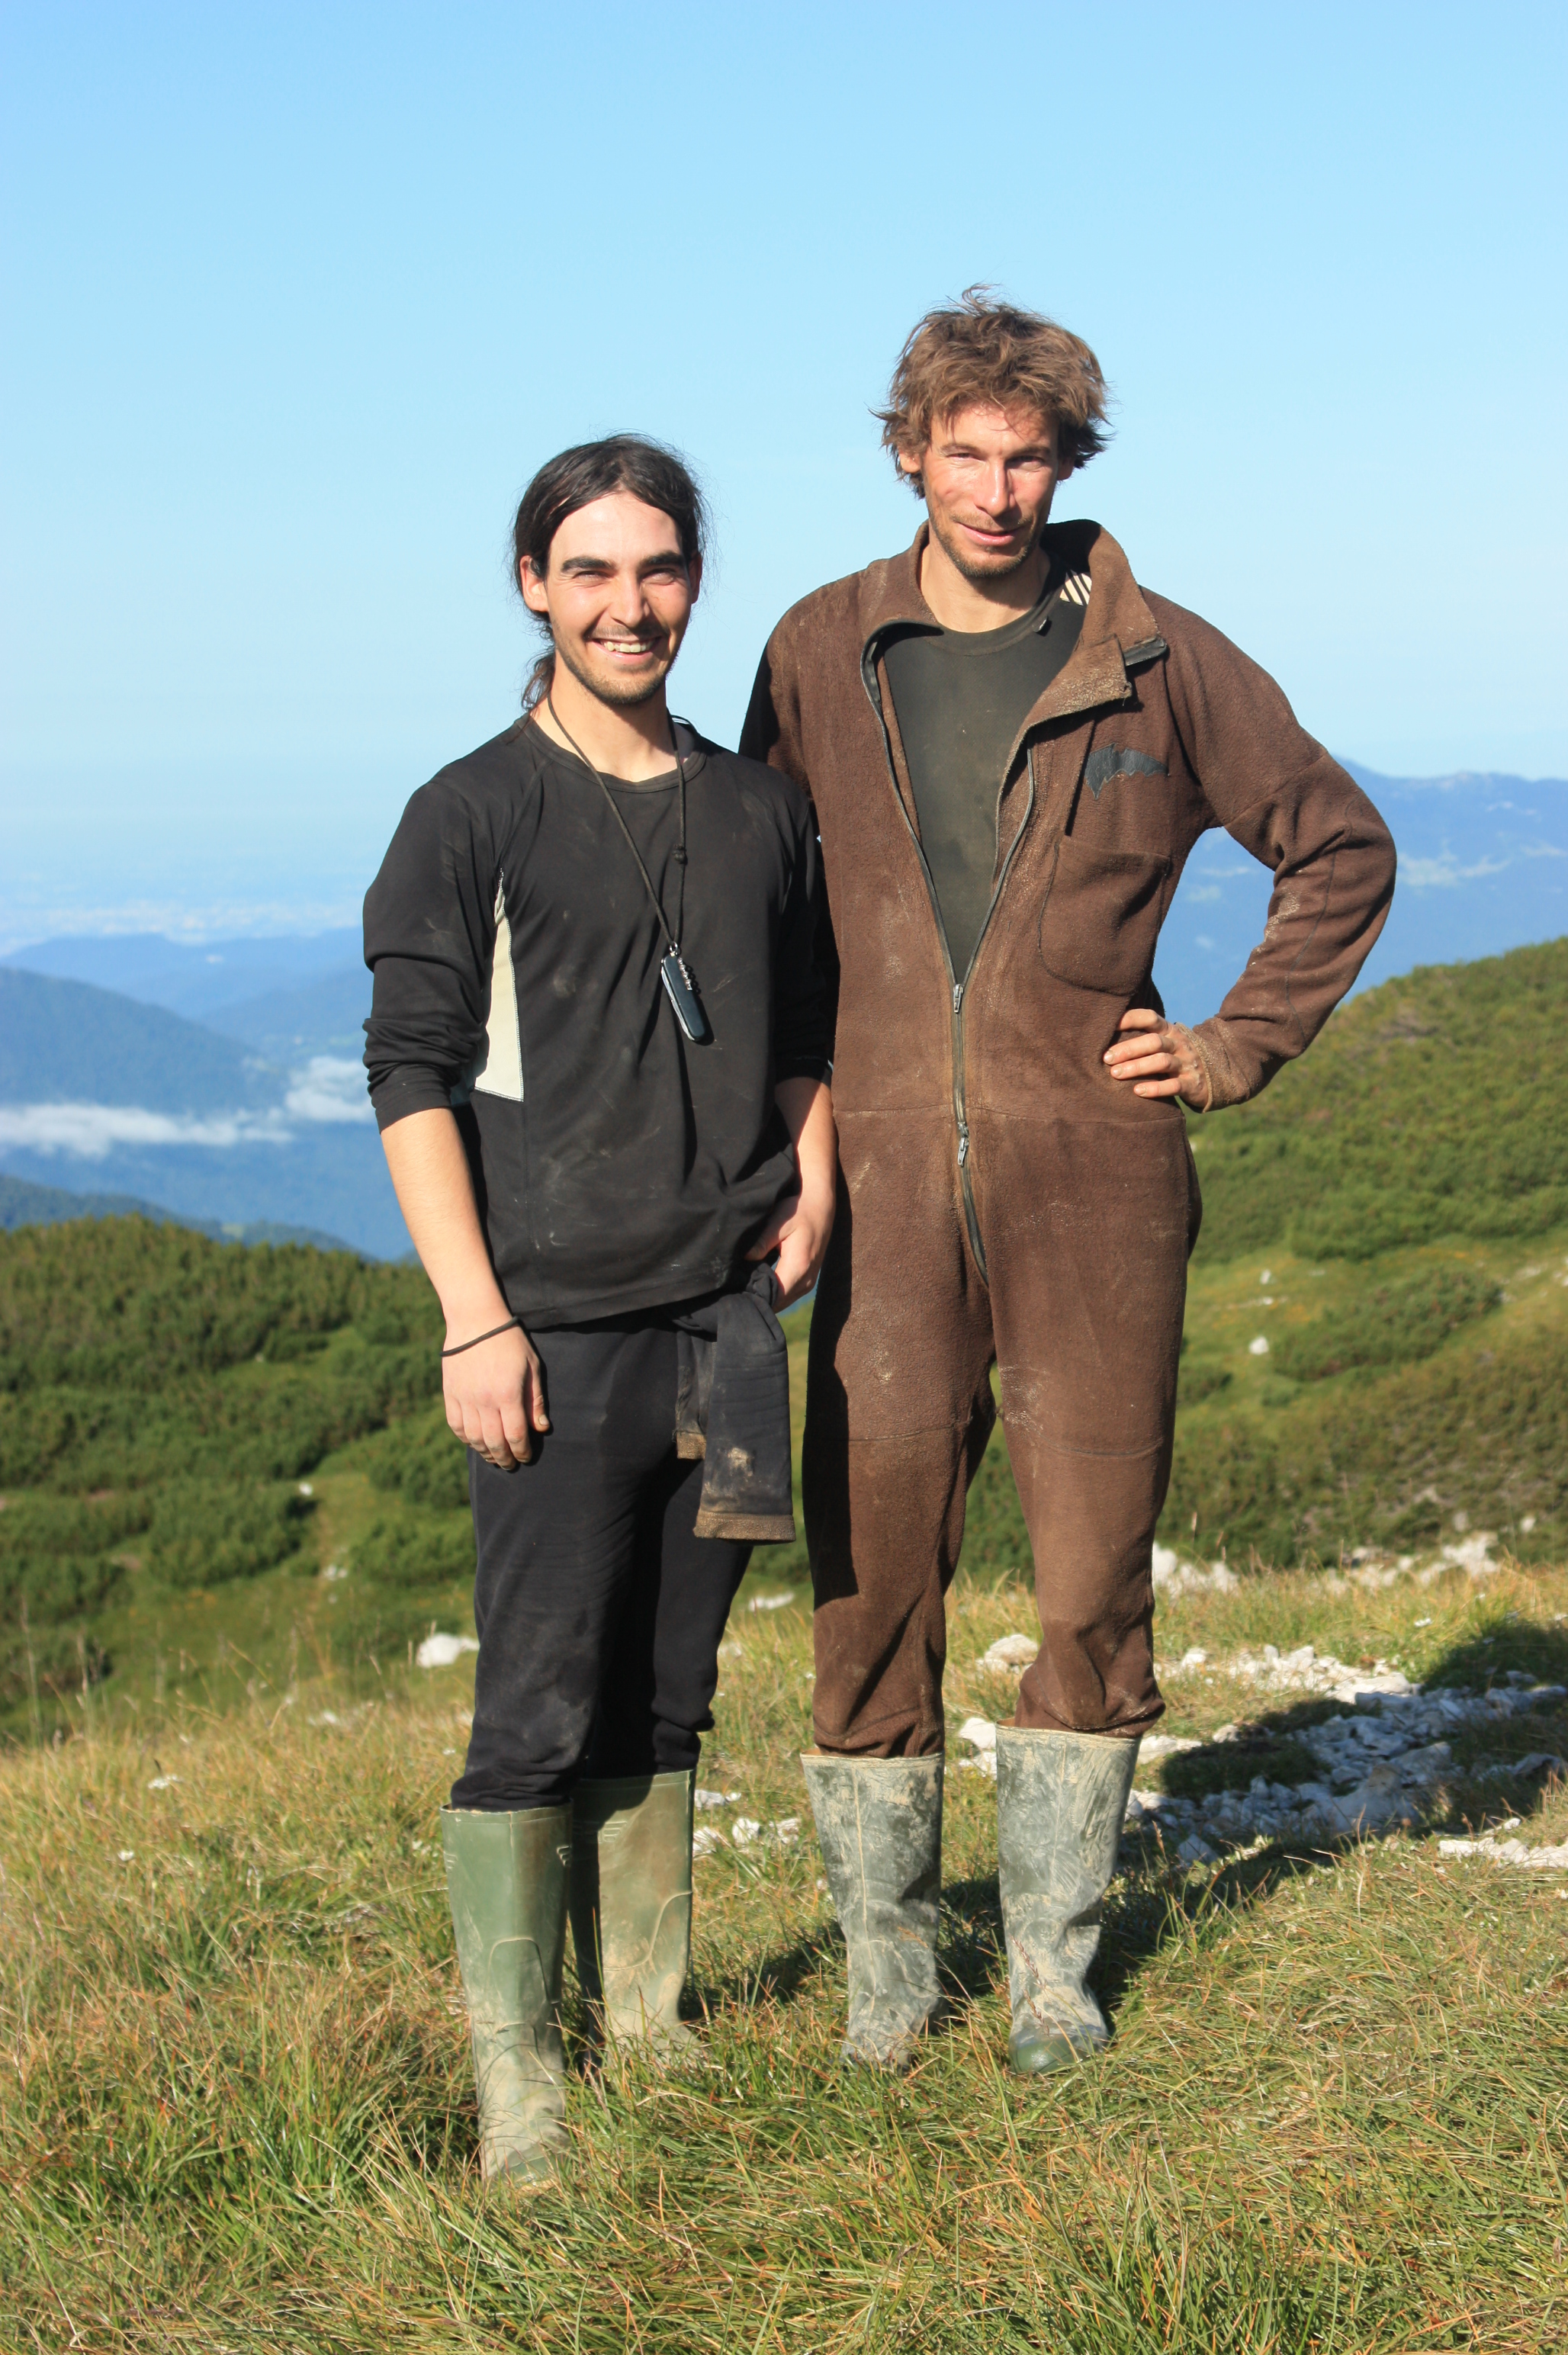
\includegraphics[width=\linewidth]{2011/discoveries/2011-08-05-07.50.41-Gergely Ambrus-Canon450D-IMG_0899-Plateau--orig.jpg}} 
 \caption{Iztok Možir and Gergely Ambrus managed to descend the muddy \passage{Stuck in Paradise} pitch and discover \protect\passage{Lost Miles} and \protect\passage{Penitence} below. \pic{Gergely Ambrus}} \label{izi gergely}
\end{marginfigure}

The \passage{Penitence} crawl\sidenote{originally \textbf{Knee Killer}} takes the
draught to a boulder choke, and includes some clean white stalagmites
(the first seen in \passage{Tolminski Migovec}) and stalactites. The entirety of
\passage{Penitence} is crawling in passage with a maximum height of one
metre. Midway along \passage{Penitence} a boulder choke is passed, with a
collection of approximately half a dozen white stal columns 20-30cm
high. \passage{Penitence} ends in a boulder choke, which was passed to lead
to \passage{Salvation}, which ends in two ways on. The first branch of
passage ends at a sandy dig with no draught; the other is (what appears
to be) an easily passable squeeze, at the end of an ascending passage,
with a howling draught. One can hear a considerable roaring at the
squeeze which is possibly water. Exploration was halted at an open lead
by lack of time, after 349 m of passage from the bottom of \passage{Stuck
in Paradise}. From the start of the \passage{Serenade} climb, development
to the current end of \passage{Penitence} is almost perfectly South-East in
direction and 500 m in plan length.

Until the discoveries this year, \passage{Vrtnarija} almost exclusively
resided in a band of rock less than 200 m wide and inclined at 70
degrees. Almost all the horizontal development was confined to
`North-South' development (actually 330 degrees true) in this band. The
new phreatic levels off \passage{Kamikaze} have developed hundreds of
metres to the South and East, seemingly unconstrained by this geomorphic
feature. They have taken the actively pushed cave passage into entirely
blank mountain, and underneath the massive drainage basin formed by the
\passage[mountain]{Kuk}-\passage[refuge]{Razor} valley. As of yet, this passage has been entirely dry, but
with a seemingly increasing draught.

\passage{Wonderland}, and the \passage{Kamikaze} extensions, were left fully
rigged as this area is almost totally dry. The exploration front is now
a considerable number of hours of caving from camp, and the lack of
accessible water is a logistical difficulty in staying hydrated.
However, this entire region discovered so far is completely weather
independent.

In total, 1.383 km of passage was found in the continuing exploration of downwind \passage{Kamikaze}.


\subsection{Other Leads}

A choke near camp, at the end of \passage{Friendship Gallery} (\passage{Lower
Pleasures}), was dug and passed to a 28 m pitch (\passage{2nd Time Lucky})
leading to continued small passage. 88 m of new passage has been found.
It is hypothesised that this passage may be the natural continuation of
the older \passage{Friendship Gallery} phreatic, before the vadose
development of \passage{Big Rock Candy Mountain} occurred.

\passage{Big Rock}, the 74 m pitch at the end of \passage{Friendship Gallery} was
known to have a window from its first descent in 2003. Recent
inspection with modern high powered lights have revealed that it is more
that we are descending in the side shaft, and that the main chamber is
still to be gained! The chambers are separated by a wall of rock about
20 m off the floor of the known pitch. A considerable volume of water
can be heard falling down in this other part of the pitch. We have no
idea where this water goes or where it could be coming from, though it
was hypothesised (in 2003) that water from \passage{Big Rock Candy
Mountain} may combine to form the \passage{Soda Stream}. A drill battery was
expended in starting a high traverse in the process of gaining the
window. As \passage{Big Rock Candy Mountain} has developed in a long rift
and we abseil down the near end, the horizontal distance to be gained is
large, perhaps 30 m.

\tweet{11:23AM Aug 12, 2011}{Final survey data entered! This year we found 2.229km of cave taking Vrtnarija to 11025/888m! More info... }

A bolt climb was made in the \passage{Queen's Bed Chamber}, using an
electric drill, 8 mm rawl bolts and a Raumer `stick-up'. Progress was
halted by the muddy layers in between the bands of good limestone. In
order to reach the hypothesised continuation of the phreatic passage, a
further 10 m of climb is needed with a solution to this technical
difficulty.

A bolt traverse was made to one of the windows on \passage{Cheetah}, and
was found to be a small abandoned inlet cascade.

The oxbow just at the beginning of \passage{Prince Consort Road} (just
beyond the roped traverse past the inlet, on the right) was pushed to a
tight inactive rift that leads upstream about 30 m and terminates in a
small chamber. Further climbing upstream is possible. This was not
surveyed.

Windows in the \passage{Albert Hall} and \passage{Minotaur Rift} were inspected,
climbed, and found not to continue.

\subsection{October M2 / Kavkna Jama}

A weekend trip with the JSPDT in October 2011 to \passage{M2}/\passage{Kavkna Jama}
brought back 245 m of survey data from discoveries over 2009-2011,
adding 100 m of depth to \passage{M2} and bringing the closest approach
between \passage{Vrtnarija} and \passage{Kavkna Jama} to 4 m (with a +- 30 m
estimated error of the 1.4 km unclosed loop). The lead ends at an easily
dug mud floored bedding plane, leading off into a tight rift, with an
extremely strong draught. The trend of the cave passage is Northerly,
towards the \passage{Captain Kangaroo} area of \passage{Vrtnarija}. Even if \passage{M2}
misses the closest point, \passage{Dark Tranquillity}, it is hoped that it will
intersect another of the \passage{Captain Kangaroo} shaft series at this depth
(\passage{Olympic Rift}, \passage{Dangermouse}).

\tweet{2:34PM Oct 23, 2011}{All safely down from mount.Last team back to hut 0630. No connection, but terminal rift pushed, dig dug and all from last 3yrs surveyed!}



\begin{pagefigure}
\checkoddpage \ifoddpage \forcerectofloat \else \forceversofloat \fi
   \centering
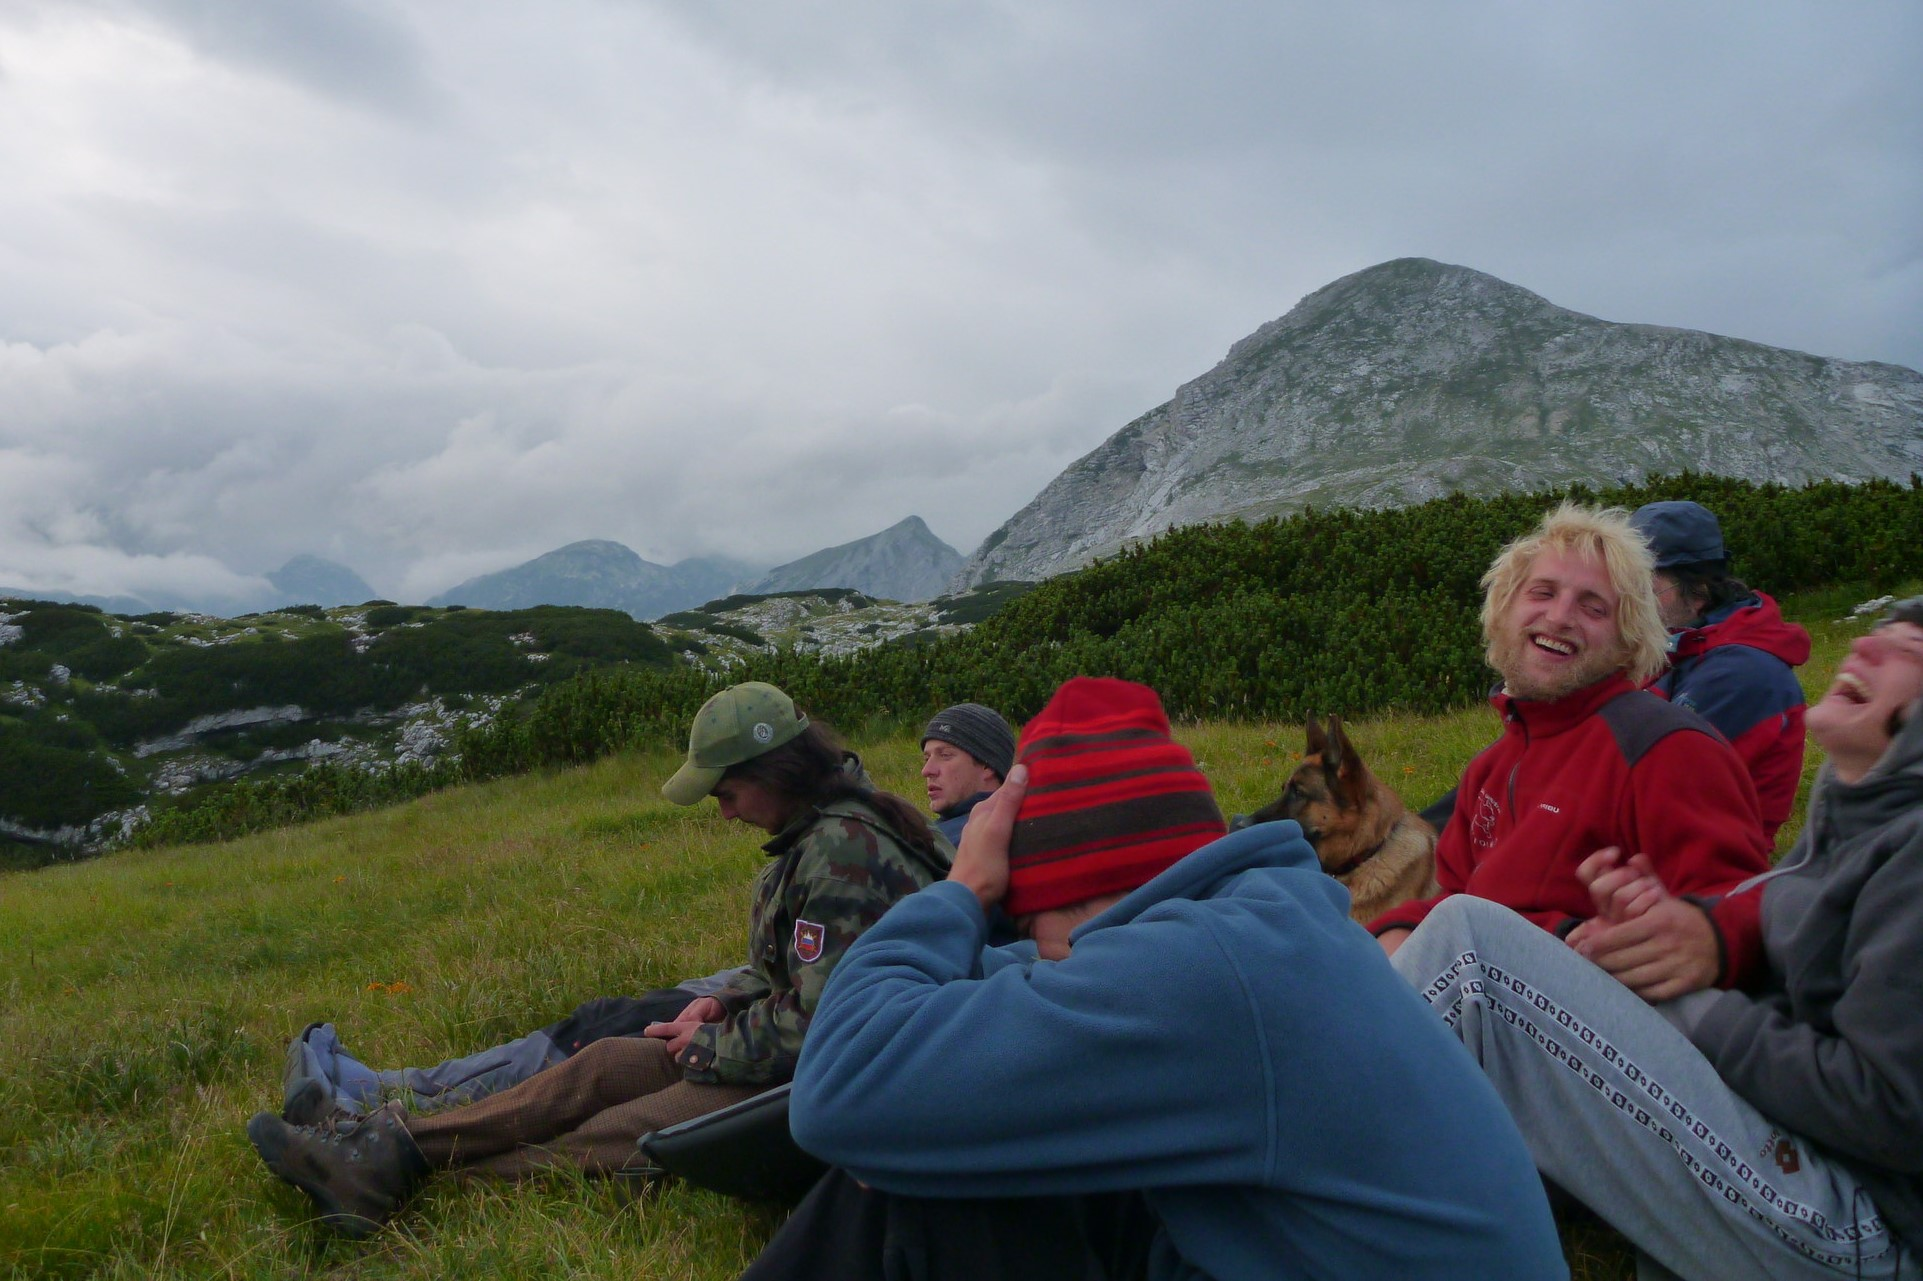
\includegraphics[width = \textwidth]{2011/discoveries/2011-07-30-19.09.31-Grega-Panasonc DMC-FT2-028--orig.jpg}
\caption{Shared laughter at sunset spot. \pic{Grega Maffi}} \label{group sunset 2011}
\end{pagefigure}
